\chapter{Backup Workload and Data Deduplication}
\label{BW}

As more and more backup systems opt to take advantage of data deduplication techniques, the variability in performance is becoming an issue. 
The cause of this variation can be categorized into two factors, \emph{systemic variation} and \emph{input variation}. Systemic variation is caused by the use of different algorithms and techniques as well as the underlying hardware deployed in the deduplication systems. The input variation is caused by different characteristics of the input datasets. The systemic variation is critical from the deduplication system designers' and vendors' perspectives since it allows them to compare two systems directly. However, the input variation is typically more critical from the customer's perspective when evaluating the potential benefits of data deduplication for different types of datasets.  

Current metrics for characterizing the datasets for data deduplication are overly simplified and often inaccurate. For example, the compression ratio ($\mathit{CR}$) is typically estimated using the \emph{average data change rate} ($\overline{\mathit{dcr}}$), which is the percentage of data change. Let $R$ be the required retention period. Assuming a full backup per unit time, the compression ratio is simply: 
\begin{equation}\label{dcr_est}
\mathit{CR}= \frac{\mathrm{Compressed\ Size}}{\mathrm{Uncompressed\ Size}}=\frac{1+(R-1)\cdot \overline{\mathit{dcr}}}{R}. 
\end{equation}
This model provides a simple estimation of the compression ratio but it can also be very inaccurate. We observed over 35\% error using the $\overline{\mathit{dcr}}$ to characterize one of our datasets. One of our main contributions is providing a new set of metrics and models that allow much more accurate compression performance predictions to be made. In five out of six cases we test, the error reduction was over 50\% when compared with the $\overline{\mathit{dcr}}$ method.  

The main performance metrics for data deduplication systems are the compression ratio and the read/write throughput. While the latency could also be an issue for virtual machines, it can be mostly masked by high level caching and prefetching mechanisms. Unless specified otherwise, we use the term \emph{performance} to represent both the throughput and compression together. 

The throughput of the system is heavily dependent on both system and input factors. Thus, it is difficult to determine if one dataset outperforms the other in terms of throughput. However, there are features of datasets that are likely to benefit throughput in most systems. One obvious one is the compression ratio itself. A highly compressible dataset has lower IO requirements which in turn improves the throughput in most systems. The compression ratio is the most influential factor in determining the throughput. However, there are also other factors, such as spatial locality of the data segments and bursty arrival rates, which we examine in this paper. 

%%Contribution
Our main contribution in this paper is to provide a framework to characterize the input dataset for data deduplication systems. We 1) show that different datasets behave with a unique pattern that is quantifiable. Furthermore, we 2) provide analysis on how this pattern affect the deduplication system performance. As part of the framework, we 3) provide classification of segment types and their relations. We further provide parameters to show how the \emph{composition} of these segment types change over time. 

\section{System Components}\label{sys}
%data component
The input data itself is another system component that affects the performance. 
To understand how the dataset affects the performance, it is described in terms of how the data components can be separated once it is deduplicated. 
The segments, regardless of how they are defined, are the smallest units of data in data deduplication. 
Therefore, we define data as a sequence of segments rather than contiguous bits or characters. 
In this work, we show that the distribution of these different segment types completely describes how the dataset affect the deduplication performance.

\subsection{Queuing Model}
The system can be viewed as simple open queuing system with three servers as seen in \CHP~\ref{BG}. We make very little assumptions of particular algorithms deployed. However, the functionality of each stage we have described in \CHP~\ref{BG} exists in all conventional deduplication systems. 
In this system, the arrival rate of segments at the \emph{content dictionary} is assumed to be exponentially distributed with the mean of average service rate at the \emph{content generator}. The probability of the arriving segments to be found in the dictionary is equal to the compression ratio in which case it can by pass the \emph{content store}. If we assume that each outcome is independent, the arrival rate at content store is also exponentially distributed. However, we show that this is not true and is one of the factors that affect the throughput of the system.  

\subsection{Segment Classification}

\begin{figure}[!t]
\centering
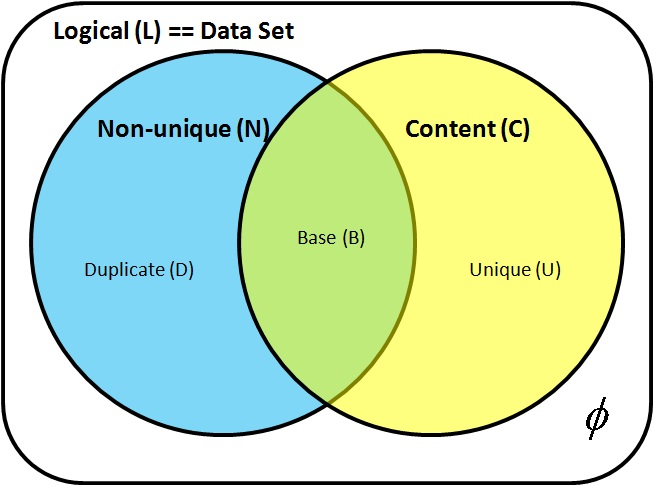
\includegraphics[width=3in]{figure/dedup/seg_classification.jpg}
\captionsetup{format=myformat}
\caption{Venn Diagram of Segment Sets. The \emph{logical segments} which is equivalent to the \emph{dataset}, can be grouped into two separate sets $N$ and $C$. The elements of $N$ are segments whose content occurs more than once in the dataset while the elements of $C$ are segments that must be stored in order to ensure no content information is lost from the dataset.}
\label{seg_class}
\end{figure}

We first define data segment as a tuple of \emph{offset} and \emph{size} within a dataset. Therefore every segment is uniquely identifiable regardless of its content. The only constraint under this definition is that the size of the data segment must be less than or equal to the size of the dataset. Also, the content of the data segment must exist within the dataset. There are no other restrictions to what may be defined as a segment. A dataset is then a mere concatenated sequence of data segments.

We begin classifying the data segments by defining the \emph{logical segments} which is the set of all segments from which you can reconstruct the original dataset through reordering only. Under this definition, a \emph{dataset} is nothing but an ordered list of logical segments. We also define \emph{unique segments} and \emph{non-unique segments}. The unique segments are a set of segments whose content is unique across the logical segments. Obviously the non-unique segments are the segments whose content is repetitive across the dataset. These non-unique segments have a unique property called the \emph{degree of repetition} which represents number of  times a particular content exist within a dataset.

From the perspective of the data deduplication system, the segments are really divided into segments whose contents must be stored and segments which can be represented only as a reference to an already stored segment. We further classify segments as either the \emph{content segments} or the \emph{duplicate segments} based on whether the content of the segment is required to reconstruct the logical segments. The content segments can be duplicated and reordered to construct the original dataset given the ordering information of contents. The duplicate segments are simply redundant contents whose only new information is the order of the content.

It is obvious from the two classifications that the duplicate segments must be the non-unique segments while the unique segments are content segments. This is shown in the \figurename~\ref{seg_class}. As shown in the figure, there exists an intersection of non-unique segments and the content segments that are called the \emph{base segments}. The base segments are minimum set of segments whose contents that must be stored to allow the deduplication system to reconstruct all the non-unique segments.

Therefore, the base segments, the unique segments and the duplicate segments are three sets of segments that are disjoint and whose union is the logical segments. A segment at any given time must be a member of one and only one of these sets.

We also define a relational parameter between these sets.
\begin{definition}[$\mathit{scr}$]\label{scr}
Segment compression ratio. $\mathit{scr} = \abs{C}/\abs{L}$ where $L=\{\mathit{logical\ segments}\}$ and $C=\{\mathit{content\ segments}\}$. 
\end{definition}

The $\mathit{scr}$ obviously represents how much of the data is actually redundant in terms of segment count. Typical data deduplication systems have some bounded segment size which ensures that $\mathit{scr}$ closely reflects the actual data reduction. 

\section{Description of the Experimental Datasets}\label{dss}

\begin{figure}
\centering
\subfloat[exchange]{\label{ex}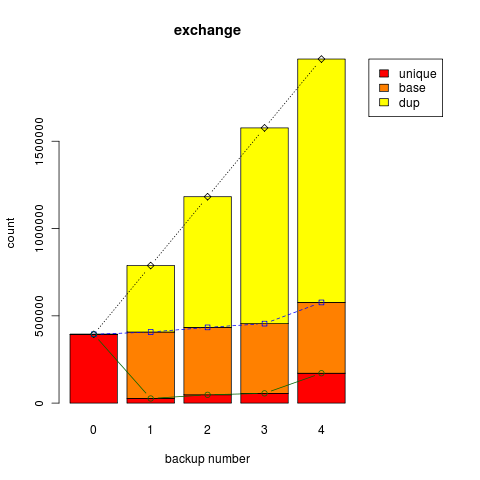
\includegraphics[width=0.5\textwidth]{figure/dedup/full011}
}
\subfloat[exchange\_is]{\label{ei}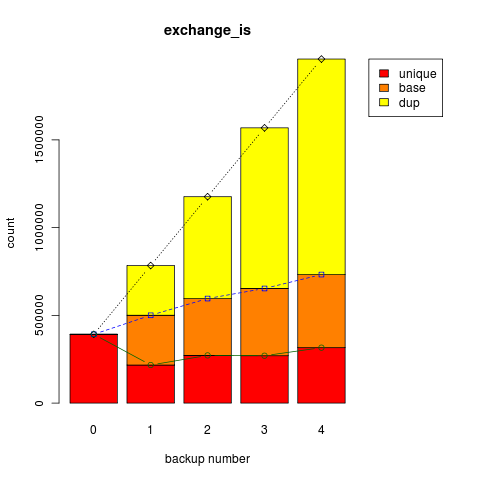
\includegraphics[width=0.5\textwidth]{figure/dedup/full012}}\\
\subfloat[exchange\_mb]{\label{em}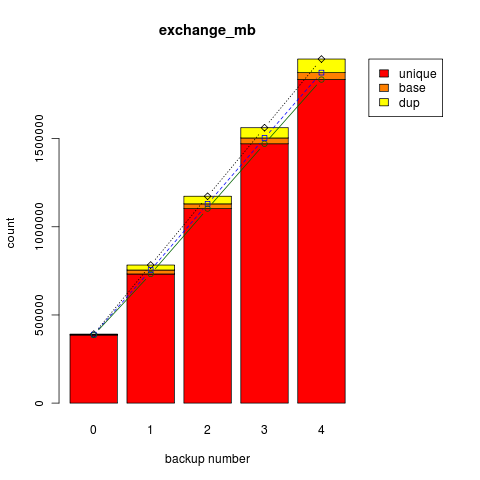
\includegraphics[width=0.5\textwidth]{figure/dedup/full013}}
\subfloat[fredp4]{\label{fp}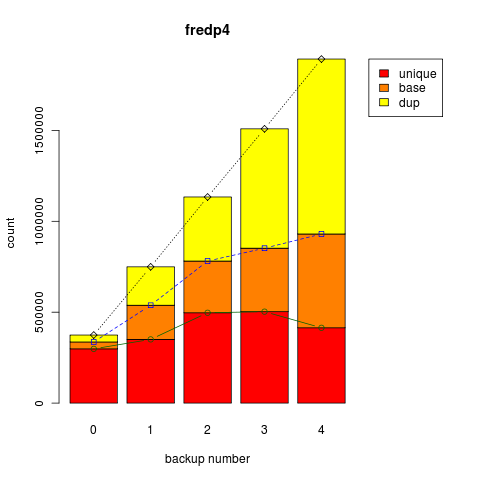
\includegraphics[width=0.5\textwidth]{figure/dedup/full014}}
\end{figure}

\begin{figure}[!t]
\ContinuedFloat
\centering
\subfloat[fredvar]{\label{fv}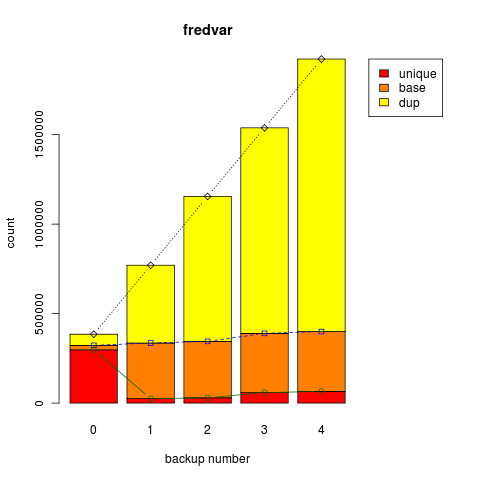
\includegraphics[width=0.5\textwidth]{figure/dedup/full015}}
\subfloat[workstation]{\label{ws}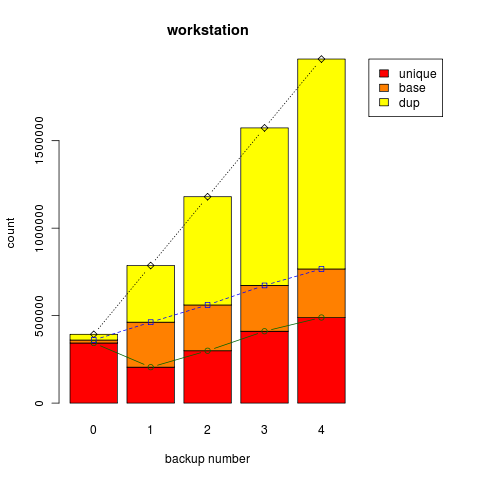
\includegraphics[width=0.5\textwidth]{figure/dedup/full016}}
\captionsetup{format=myformat}
\caption{Composition of segments for different datasets. Graphs show how the composition of segments changes over time as weekly full backups are deduplicated.}
\label{fig_sim}
\end{figure}

\begin{table}[!t]
\centering
\begin{tabular}{c||c c c}
\hline
\bfseries Dataset 	&\bfseries Number of	&\bfseries Compression 	&\bfseries Throughput	\\
 			&\bfseries Segments	&\bfseries Ratio 		&\bfseries (MB/s)		\\
\hline\hline
exchange 		&1,970,836			&0.294			&44.72			\\
exchange\_is	&1,960,555			&0.377			&42.60			\\
exchange\_mb 	&1,951,271			&0.973			&27.20			\\
fredp4		&1,892,285			&0.502			&39.78			\\
fredvar		&1,922,420			&0.209			&48.36			\\
workstation		&1,966,577			&0.403			&38.92			\\
\hline  
\end{tabular}
\captionsetup{format=myformat}
\caption{Datasets. Six datasets with the size of the logical segment set and two performance metrics of interest.}
\label{ds_t}
\end{table}

\begin{table}[!t]
\centering
\begin{tabular}{c|c|| c| c}
\hline
\bfseries Parameters 	&\bfseries Value		&\bfseries Parameters 	&\bfseries Value		\\
\hline\hline
Content Generation	&Content			&Minimum 			&4KB				\\
Method			&Based			&Segment Size		&				\\
\hline
Average			&8KB				&Maximum			&16KB			\\
Segment Size		&				&Segment Size		&				\\
\hline
Storage Maximum	 	&50MB/s 			&Maximum Network	&100MB/s			\\
Throughput (sequential)	& 				&Throughput		&				\\
\hline
Content Dictionary		&100,000			&Hash Function		&SHA1			\\
Cache Size			&entries			&for Segment ID		&(160 bits)			\\
\hline
\# of Bloom Filter 		&4				&Bloom Filter Size		&1,000,000			\\
Hash Functions 		&				&				&entries			\\
\hline
\end{tabular}
\captionsetup{format=myformat}
\caption{Experimental deduplication parameters.}
\label{ex_t}
\end{table}

Six different datasets shown in \tablename~\ref{ds_t} were used in our evaluation. Due to privacy concerns, only the SHA1, size and the backup order of the segments were made available.\footnote{The actual data provided also contained compressed size of the segment, stream offset which represents where the segment is located in the original dataset. The compressed size is unused since the local compression of segments is not of interest in this study and stream offset is redundant information which can be deduced from the order and the size of the segments.} We refer to this data as \emph{segment trace}. 

The \emph{exchange}, \emph{exchange\_is} and \emph{exchange\_mb} datasets are all Exchange server data encoded in different ways. The \emph{fredp4} dataset contain a revision control system data and \emph{fredvar} contain data from /var directory in the same machine. The \emph{workstation} dataset contains data from the home directories of several users.  

The segment trace is not of the entire original dataset. Unfortunately, the data presented to us were of the data that is truncated from a larger dataset. Although a truncated dataset is used, it does not effect the methodology presented in this paper. This is because we characterize the datasets based on how deduplication system processes them. There are only a specific range of data characteristics from deduplication system's point of view. And these truncated datasets are used to show where in this range a particular dataset may lay. We could easily have done same analysis with the synthetic traces since their characteristics cannot lay outside this range regardless of how we generate the trace. 

The system parameters for data deduplication system is described in the \tablename~\ref{ex_t}. The cache size for the \emph{content dictionary} is kept reasonably small to capture the effect of cache misses. Since the maximum raw throughput of the system is IO limited at 50MB/s, you can see that the throughput of different datasets vary from being close to the maximum throughput to about 50\% of that throughput. 

As mentioned earlier, there is a strong linear relationship between the compression ratio and the throughput. The sample correlation coefficient, $r_{ct} = -0.98$ (where $c=compression\ ratio$ and $t=throughput$), suggest that higher compression (lower compression ratio) results in higher throughput. While it may seem that compression ratio is the dominant factor in determining the throughput since the two are so highly correlated, the system for which the throughput numbers are reported are \emph{in-line} deduplication systems where all segments must be compared against the content dictionary before it can be stored on the disk. Therefore, the elimination of duplicate segments not only results in dictionary update but also additional disk writes. In systems where data may already all be written to the disk before being looked up in dictionary may not perform in exactly the same manner. Therefore, we concentrate more on dictionary access pattern to analyze potential throughput concerns.

The segment trace contains 5 weekly full backup information of 6 different datasets and 5GB of each full backup. Therefore, all data presented in \tablename~\ref{ds_t} are of the same size at 25GB. The variation in number of segments is due to variation in average segment size. Compression ratio provided in the table is compression due to data deduplication process only and does not include additional compression provided by local compression of segments using traditional data compression tools. 



\section{Data Characterization}\label{result}

An obvious and perhaps the most important data characteristic for data deduplication is amount of redundancy. Two datasets of equal redundancy would yield in similar compression assuming the content generation was done in a reasonable manner. However, they could perform very differently depending on the other aspects such as locality of segments and fragmentation due to elimination of duplicate segments. The difficulty in characterizing workload of data deduplication is that the characteristics is actually dependent on the contents. While access patterns and physical attributes such as size of files tends to follow a well known distributions in a large scale~\cite{riska:2009, leung:2008}, contents themselves are random in nature due to human factor and different encoding deployed by different applications.

\subsection {Composition of Segments}

\begin{figure}[!t]
\centering
\subfloat[Base segments]{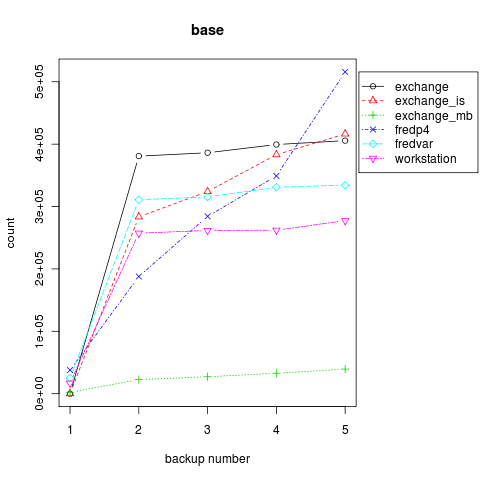
\includegraphics[width=0.5\textwidth]{figure/dedup/full005}
\label{bs}}
\subfloat[Duplicate segments]{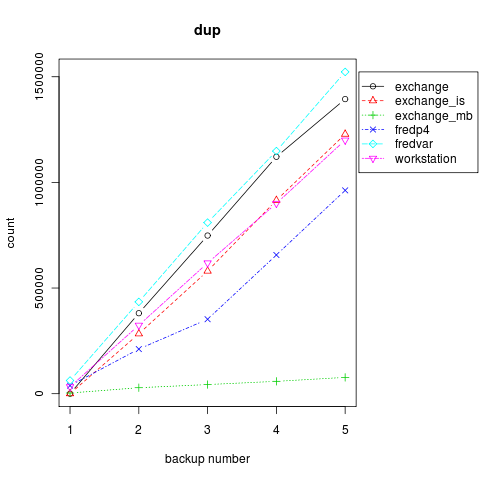
\includegraphics[width=0.5\textwidth]{figure/dedup/full002}
\label{dups}}\\
\subfloat[Average references]{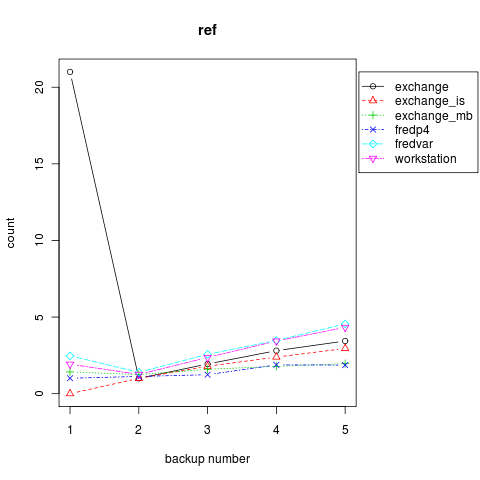
\includegraphics[width=0.5\textwidth]{figure/dedup/full009}
\label{ar}}
\captionsetup{format=myformat}
\caption{Comparison of data sets. Number of references are simply $|D|/|B|$. Therefore, \emph{exchange\_is} and \emph{frep4} show lowest average number of references since their number of base segments increase with the number of duplicate segments. For all other segments, the number of base segments stay relatively steady indicating that same portion of the data is changing over and over again.}
\label{data_comp}
\end{figure}

\figurename~\ref{fig_sim} shows how the composition of segments, as defined in \figurename~\ref{seg_class}, changes over time for each dataset at a full backup granularity.  The composition of the segments is quite different for all datasets. In the figure \emph{backup number} represents accumulated number of full backups stored in the system. We make a few observations from the composition.

\begin{observation}\label{1}
Amount of duplication found within a single full backup is negligible compared to the duplication found across the full backups.
\end{observation}

This is an observation also made by other deduplication works on backup data~\cite{kruus:2010}. This observation allows us to look at the changes in the composition of segments as results of deduplicating a full backup instance against other instances of full backup. While non-zero unique and base segments at backup number 0 in \figurename~\ref{fp},  \figurename~\ref{fv} and  \figurename~\ref{ws} indicate that there exists some inter-duplication within a backup, the amount is negligible and we ignore its effect in this paper.

\begin{observation}\label{2}
For the base segments there are two distinctive case where number of base segments increase with number of fulls as in \figurename~\ref{ei} and \figurename~\ref{fp} and case where number of base segments stay steady as shown in \figurename~\ref{ex}, \figurename~\ref{fv} and \figurename~\ref{ws}.
\end{observation}

This observation can be made more pronounced in \figurename~\ref{bs}.

The number of base segments can only increase in the absence of the deletion. Once a segment becomes a base segment, it cannot become any other type of segment. Therefore, the number of base segment can only stay steady if there is no or very little amount of new base segments are created. We can conclude that in this kind of dataset, the unique segments stays unique segments while the same set of base segments keeps getting duplicated.

Conversely, the increase in number of base segments mean that the unique segments of previous backup number is getting converted to the base segments. This happens only when a newly generate data at backup number $i$ still exists at backup number $i+1$. We assume that no base segments are generated within a full backup instance based on the observation \ref{1}. We call this rate of conversion \emph{base generation rate}($bgr$) which is bounded by the number of unique segments in previous backup number and is larger than or equal to 0.

We formally define $bgr$ below.

\begin{definition}[$bgr$]
Rate at which unique segments are converted to base segments. $bgr_i=\frac{|B_{i+1}|-|B_i|}{|U_i|}$ where the subscripts represent the backup number. We define $bgr$ to be average value of $bgr_i$, $bgr = \frac{\sum bgr_i}{max(backup number)}$.
\end{definition}

\begin{observation}\label{3}
The number of unique segments either increase steadily as shown in \figurename~\ref{em} and \figurename~\ref{ws} or stay relatively steady as in the rest of the figures in \figurename~\ref{fig_sim}. While the number of unique segments can decrease, it does not happen very often.
\end{observation}

The number of unique segments, $|U|$, at backup number $i$ is increase by amount of unique segments generated by that particular full backup and is decreased by amount of unique segments at backup number $i-1$ converted to base segments\footnote{Conversion to duplicate segments is also possible but is ignored due to observation \ref{1}.} at backup number $i$. Since the amount of decrease in $|U_{i+1}|$ is $|U_i|\times bgr_i$, we also need to define a parameter to represent the increase in $|U|$, \emph{unique segment ratio}(usr). This ratio does not represent the changes in the number of unique segments, $|U|$, since there is also conversion of segments from unique to base.

\begin{definition}[$\mathit{usr}$]
Relative amount of unique segments within a full backup. $usr_i = \frac{|U_{i+1}|-|U_i|(1-bgr_i)}{|L_{i+1}|}$. We define $\mathit{usr}$ to be average value of $usr_i$, $usr = \frac{\sum usr_i}{max(backup number)}$.
\end{definition}

From the definition of $\mathit{usr}$ it is obvious that we cannot simply determine the rate of unique segment generation from looking at the changes in $|U|$. However, since it is possible to determine the $bgr$ from also looking at the changes in number of base segments, $|B|$ which in turn allow us to calculate $\mathit{usr}$. Since increase in $|B|$ is only possible due to $bgr$, if increase is very small, we can assume that $bgr\simeq0$. This allows us to think that $usr_i=U_{i+1}-U_i$ which means that unique segments in backup number $i$ no longer exists in backup number $i+1$ or else they would have become base segments. This pattern is most pronounced in \figurename~\ref{ws}. Intuitively, the pattern suggests the existence of a small and heavily updated \emph{working set} within the file system as suggested by~\cite{soundararajan:2010}. Similar analysis could applied to \figurename~\ref{em} where almost the entire dataset is a working set. 

Cases where $|B|$ actually increase with the backup number, $bgr$ represents the rate at which new data becomes part of \emph{non-working set}. It suggest that part of the working set becomes stable over time and becomes base on which future segments are deduplicated. Extreme case is shown in \figurename~\ref{fp} where the effect of $bgr$ starts to outweigh the effect of $\mathit{usr}$ and the number of unique segments actually decrease. This is the most desirable case for the data deduplication where amount of data to be store grows sub-linearly and therefore more scalable in terms of backups you can store. It will also be shown that the throughput also tends to be higher in these cases for similar compression.

Cases seen in \figurename~\ref{ex} and \figurename~\ref{fv} suggest that there exists only a small change between the backups. While this is also a desirable case for data deduplication, it may also be argued that for a storage system with such little activity, a longer period of incremental backups could provide similar performance. 

The logical size, $usr$ and $bgr$ of a dataset completely describes the dataset as long as there is no deletion involved. Furthermore, they do not vary as much as $dcr$ over time. Therefore a aggregated values of $usr$ and $bgr$ are much better choices of parameters to describe a dataset. They show how much of new data is generated ($|L|*\overline{\mathit{usr}}$), how much of that data will be changed again before the next full ($1-\mathit{bgr}$). Together, they allow you to calculate the compression ratio at time $i+1$ by following these steps. 
\begin{enumerate}
\item{$|B_{i+1}|=|U_{i}|*\mathit{bgr}_i+|B_i|$.}
\item{$|U_{i+1}|=|L_{i+1}|*\mathit{usr}+|U_i|(1-\mathit{bgr}_i)$.}
\item{Calculate $|D_{i+1}|$ and $\mathit{scr}$ from above two values.}
\end{enumerate}

\subsection{Segment Run Length}

\begin{figure}[!t]
\centering
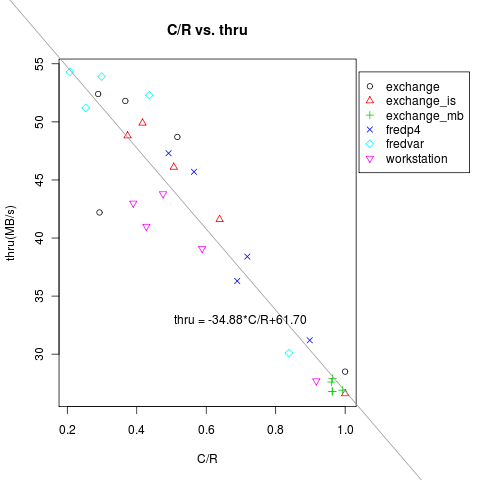
\includegraphics[width=0.8\textwidth]{figure/dedup/full018}
\captionsetup{format=myformat}
\caption{C/R vs. Throughput. The accumulated compression ratio of each dataset at each full backup is plotted against the throughput for that particular backup window. You can observe that the throughput increases as the accumulated compression ratio decreases even though every full backup is equal in size.}
\label{compthru}
\end{figure}

\begin{figure}[!t]
\centering
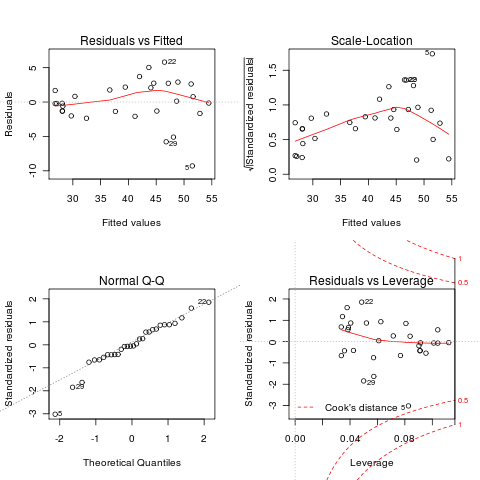
\includegraphics[width=0.8\textwidth]{figure/dedup/full019}
\captionsetup{format=myformat}
\caption{Analysis of C/R vs.throughput. The top left graph shows that while the regression is a good fit, data around throughput value of 40MB/s to 50MB/s tends to out perform expected throughput. Top right graph shows square root of residual error. The backup instance 5, 22 and 29 show a large deviation (from exchange, fredvar and workstation datasets respectively). The lower left graph shows that the residual errors are more or less normally distributed with the exception of 4, 21, 29 (from exchange, exchange\_is and workstation datasets respectively). The lower right graph shows the Cook's distance. Backup instance 5 is less than 0.5 Cook's distance away and can be safely taken into evaluation.} 
\label{anal}
\end{figure}

In section \ref{dss}, we showed that the compression ratio and the throughput of a deduplication system can be highly correlated. \figurename~\ref{compthru} shows throughput vs. compression ratio of each backup instances. This graph together with \figurename~\ref{anal} shows that the compression ratio is indeed a most relevant factor in determining throughput. However, \figurename~\ref{anal} shows some skewness both in Residual vs. Fitted graph and Residual vs. Leverage graph. They suggest at other factors that affect throughput which are not simply white noise. 

\figurename~\ref{compthru} also shows a linear estimation line. One interesting observation is that there are some datasets which perform consistently better than the estimation. These are \emph{exchange\_is}, \emph{fredp4} and \emph{fredvar} datasets. On the other hand, \emph{workstation} dataset performs consistently worse than expected. 

To quantify this effect, we take look at the deviation of throughput numbers from the regression line as shown in \tablename~\ref{dev}. These numbers are not absolute deviation. These are average values of $actual\ throughput - expected\ throughput$ and removes the effect of the compression ratio from the throughput numbers. As explained in section \ref{sys}, the \emph{content dictionary} is the only place where this variation in performance due to content could occur. Note that all data are of the same size, written sequentially once. While \emph{content store} actually stores less if more segments are deduplicated, this performance difference is likely to be linear to the amount of data stored. Since we have removed this linear factor and concentrate only on the deviation, the effect must be due to on content dictionary behavior.

To evaluate the content dictionary behavior, we first look at the sequential runs of segments. A longer sequence of a run represents a sequential access of content dictionary making it easier for the dictionary cache to be a hit. A \emph{run} is simply a sequence of consecutive segments that are either unique or duplicate segments. We refer to them as a \emph{content run} and \emph{duplicate run} respectively when need to distinguish between them. \tablename~\ref{dev} shows aggregated \emph{run} data. We make following observations.

\begin{table}[!t]
\centering
\begin{tabular}{c||c c c c}
\hline
\bfseries Dataset 	&\bfseries Average	&\bfseries Max		&\bfseries Average	&\bfseries Run Len.	\\
 			&\bfseries Deviation 	&\bfseries Run Len.	&\bfseries Run Len.	&\bfseries $> 1000$	\\		
\hline\hline
fredp4		&1.532			&207400			&7.944			&57\%			\\
exchange\_is	&1.375			&392000			&15.88			&27\%			\\
fredvar		&0.852			&366200			&28.88			&76\%			\\
exchange 		&0.217			&183100			&30.53			&64\%			\\
exchange\_mb 	&-0.722			&7490			&18.6				&13\%			\\
workstation		&-3.260			&5632			&6.635			&9\%				\\			
\hline
\end{tabular}
\captionsetup{format=myformat}
\caption{Average Deviation from the expected throughput and their corresponding run length information}
\label{dev}
\end{table}

\begin{observation}
The average run length varies little across the datasets and shows little correlation to the throughput. However, the maximum run length varies significantly across the datasets and show high correlation.
\end{observation}

The correlation coefficient of maximum run length and the average deviation is $r^2 = 0.63$. It is high enough that we can safely assume there is significant correlation between the two values. The correlation coefficient of average run length and the average deviation is only $r^2 = 0.002$. The obvious reason is that the mean values of run length does not represent anything physical when the significant portions of the data lay in outlier regions. The last column of \tablename~\ref{dev} shows that the over 50\% of the segments fall in a run length of over 1000. It is interesting to note that the \emph{fredvar} and \emph{exchange} datasets suffer in throughput even though they have the highest percentage of large runs. It leads us to our next observation.

\begin{observation}
Datasets with high average run length due to many extremely large runs perform worse than cases where the run length are more evenly distributed. 
\end{observation}

The skewed run length has a negative impact on performance not because of the content dictionary but the content store. While it is obvious that less amount to be stored result in high logical throughput as described earlier, the arrival rate of segments to the content store is also important. In a simple queuing model, the arrival rate at the content store is simply $(1-p)S$ where $S$ is the throughput of the content dictionary and $p$ is content dictionary hit probability. If $p$ was uniformly distributed, that the arrival rate would simply be a function of compression ratio. However, as the skewed distribution of run length shows, $p$ of each segments are highly correlated. The effect is bursty arrivals at the content sore resulting in high queue length and lower throughput as shown in \figurename~\ref{ql}. It is shown that the effect of run length is less pronounced for datasets with higher compression ratio. The \emph{all\_miss} case is the worst case where every segment is sent to the segment store and \emph{rand} is the best case where run length distribution is uniform.
 
\begin{figure}[!t]
\centering
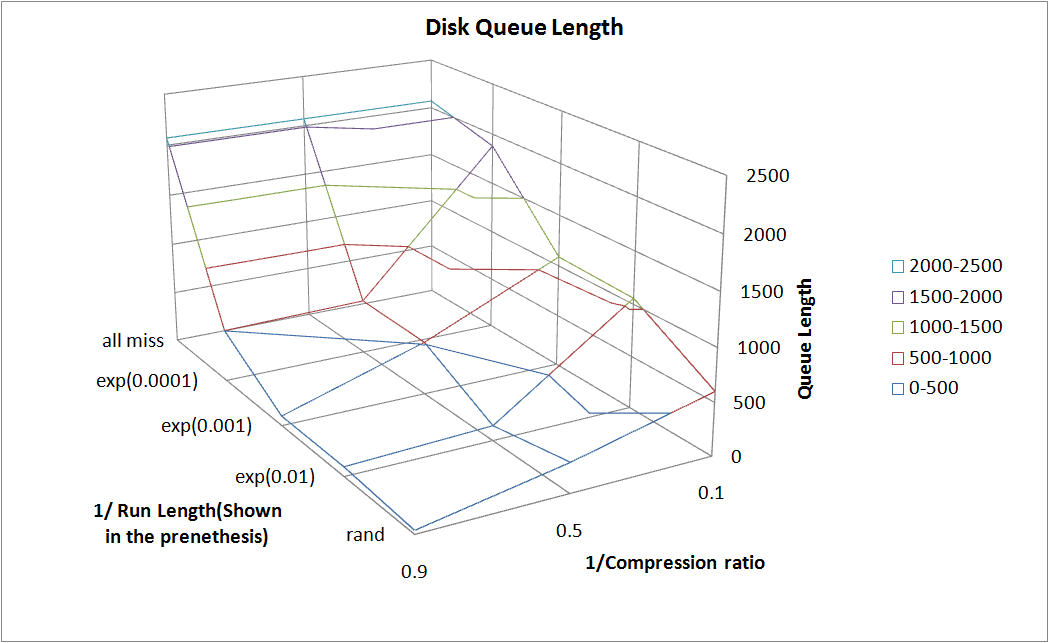
\includegraphics[width=0.8\textwidth]{figure/dedup/disk_q}
\captionsetup{format=myformat}
\caption{Run length vs. compression ratio vs. queue length.}
\label{ql}
\end{figure}

The run length analysis shows that while the throughput is highly correlated with the compression ratio, higher run length typically results in higher throughput. Additionally, skewed run length which typically results from few very long runs, results in lower throughput especially when the compression ratio is low.

\section{Applications}\label{appp}
Above analysis of composition of segments allows users of deduplication systems to collect specific statistics to predict future storage requirements. In the world of deduplication where the physical storage space and the logical segment space does not match, it is difficult to provision storage space. Extracting $bgr$ and $usr$ from the deduplicated data allow users to better predict future storage requirements. 

For the given six test datasets, we use $bgr$ and $usr$ of the first three fulls to predict the compression ratio of 4th and 5th full and compare them with the $dcr$ approach.

For example, the $bgr_1\sim 0.01$ and $usr_1\sim 0.26$ for \emph{workstation} dataset. Since $|L_i|\sim393311$,  we can predict future segment composition given backup number 2 information. \figurename~\ref{pred} shows the graph of the original workstation composition and the graph of predicted composition. Since the parameters were extracted from the backup number 1 and 2, the accuracy of prediction falls as the number of fulls increase. Of course, the accuracy of the prediction itself is also dependent on the dataset and the worst case error was observed in \emph{exchange} dataset where the $\mathit{scr}$ at backup 4 was off by just over 0.02($\sim5\%$ error). This is much better approach than simply observing the compression ratio. For \emph{fredp4} dataset the $dcr$  prediction is off in compression ratio by 0.18 ($\sim36\%$ error).

\begin{table}[!t]
\centering
\begin{tabular}{c||c c}
\hline
\bfseries datasets &\bfseries dcr	 	&\bfseries usr \& bgr	\\
\hline\hline
fredp4		&35.99\%			&3.68\%					\\
exchange\_is	&9.20\%			&2.21\%				\\
fredvar		&7.35\%			&0.21\%						\\
exchange 		&17.82\%			&5.42\%					\\
exchange\_mb 	&0.14\%			&0.20\%				\\
workstation		&3.61\%			&0.61\%				\\			
\hline
\end{tabular}
\captionsetup{format=myformat}
\caption{Compression ratio prediction error comparison}
\label{err}
\end{table}

\tablename~\ref{err} shows our approach outperforms the traditional $dcr$ approach in all but exchange\_mb dataset where the error is about the same.

Another potential application is evaluating the impact of merging two separately deduplicated data. Unless there is a reason to suspect a large similarity between the two datasets, parameters of each dataset can be superpositioned to predict the composition of combined dataset. 

A more involved application would be to filter out the \emph{working set} from being deduplicated. Various techniques exists to evaluate the working set of a storage system~\cite{lee:2009, wang:2004} which can be used to identify \emph{hot data} and pass only those deemed cold to the deduplication system. This would be especially useful for datasets with low $bgr$ where same portions of the data are constantly changing. This portion can deemed unworthy of deduplication and is backed up separately. 

The analysis of run length suggest that it maybe more beneficial for the through put if the inter-duplicate segments are ignored. That is we only evaluate duplicate segments generated between the full backups. These single or dual duplicate segments fragment the index table and potentially the contents on disk without providing any substantial gain in compression. 

Last application maybe to adjust buffer sizes at each stage of deduplication based on the run length observed to minimized skewed arrival effect. 

\begin{figure}[!t]
\centerline{
\subfloat[Real Data]{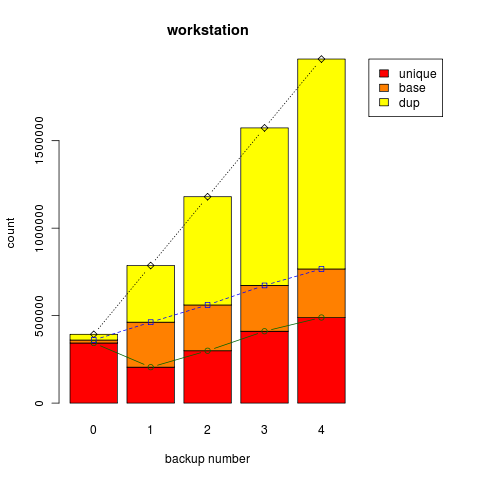
\includegraphics[width=0.5\textwidth]{figure/dedup/full016}
\label{wo}}
\hfil
\subfloat[Predicted Data]{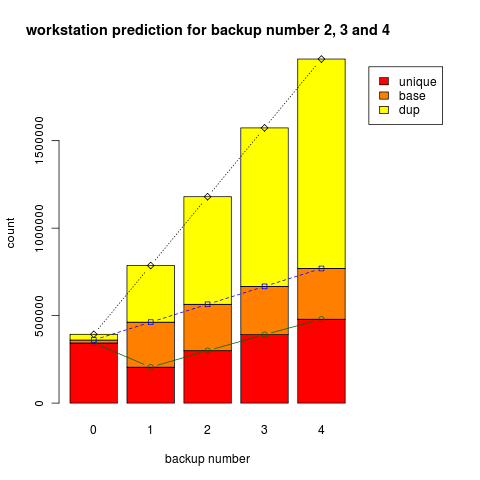
\includegraphics[width=0.5\textwidth]{figure/dedup/prediction001}
\label{wp}}
}
\captionsetup{format=myformat}
\caption{The original segment composition of workstation and the predicted values.}
\label{pred}
\end{figure}

\section{Limitations}\label{lim}
%%Assumptions - second assumption can be proven with in statistical margin.
Many deduplication systems allow the segments to be stored without duplicate detection for the better throughput~\cite{bhagwat:2009, lillibridge:2009}. This does not cause correctness issue. However, it makes predicting performance even more difficult. In this study we assume that all duplicate segments must be identified and eliminated. There has also been attempts to make better decisions on identifying the data segments from the dataset~\cite{eshghi:2005, kruus:2010, bobbarjung:2006}. We claim that the segments, regardless of how they are defined, define datasets in terms of data deduplication process. This claim assumes that different datasets will have statistically similar relative compression and performance regardless of the segmentation process. In other words, segmentation process affects different dataset in statistically similar way. For example, if dataset $A$ gained compression ratio by 10\% while losing throughput by 5\% by using the new segmentation method, than dataset $B$ is highly probable to gain in compression and lose in throughput by similar amount. While this assumption is actually verifiable, lack of datasets prevents us from providing strong statistical guarantee. However, previous analysis of segmentation algorithms~\cite{kruus:2010} as well as our own tests indicate no evidence to reject our assumption.

\section{Conclusion}\label{con}
We have shown a framework for characterizing datasets by analyzing how different datasets behave within a data deduplication system. For the datasets presented here, we show that there are classes of datasets which behave similarly.

We also show that the changes in the number of base segments is more important in terms of scalable data compression than the simple compression ratio. More specifically, a positive $bgr$ guarantees continuing reduction in the compression ratio resulting in sub-linear growth in the storage requirement. Intuitively, $bgr$ represents life time of new data. High $bgr$ means that newly created data are long lived and low $bgr$ means that they are short lived. Since $usr$ represents amount of new data created, their ratio tells you how much of the new data is transient and how much are more permanent. Generating more and more permanent data means more data to be deduplicated at each back up resulting in better compression ratio.  

We also show that the segment run length has a fundamental effect on the dictionary lookup process both in terms of the cache behavior and queuing delays, which can counteract each other in terms of throughput. More specifically, the typical belief that high average run length results in better throughput is not true. In fact, it can lower the throughput due to skewed arrival rate the content store. However, high maximum run length tends to improve performance due to good caching effect of content dictionary. Simply put, one can estimate throughput based on the compression ratio using a C/R vs. throughput regression line for a given system and can further expect the throughput to be better or worse based on the run length information.

Lastly, we showed that we can increase the accuracy of compression ratio prediction by as much as 80\%. Furthermore, we can accurately predict the composition of segments which allow us to determine the existence of frequently updated data which does not have to be deduplicated. 

%%%%%%%%%%%%%%%%%%%%%%%%%%%%%%%%%%%%%%%%%%%%%%%%%%%%%%%%%%%%%%%%%%%%%%%%%%%%%%%%
